\documentclass[12pt, a4paper]{article}
\usepackage[utf8]{inputenc}
\usepackage[cm]{fullpage}
\usepackage{fancyhdr}
\usepackage{graphicx}

\begin{document}

\title{Protolize!: A new computational tool for frequency analysis of electroencephalographic signals}
\author{Sergio Conde, Alexandre Ricardo Romariz, Carlos Tomaz}
\date{}
\maketitle

\begin{abstract}

In this research a computational tool named $Protolize!$ was developed for biological signal processing, with emphasis on electroencephalographic signals, in the time-frequency domain. The tool performs analysis using the Fourier Transform, the Short Time Fourier Transform, the Continuous Wavelet Transform and multi-resolution analysis through Discrete Wavelet Transform. It offers configuration options to choose between different kinds of windows and wavelets families. Performance and usefulness of the computational tool were illustrated by processing electroencephalography signals collected, in 47 volunteers, where alpha block phenomenon was reproduced. $Protolize!$ was implemented using Matlab® R2007b, and it’s a free tool available in a public repository. 

\end{abstract}

\textbf{Keywords}: Signal Processing, Frequency analysis, Fourier, Wavelets, software, EEG.

\section{About the authors}

Sergio Conde (sconde@unb.br), Laboratory of Neuroscience and Behavior, Department of Physiological Sciences, Institute of Biology, University of Brasilia, CEP 70910-900 Brasilia, DF,  Brazil.

Alexandre Ricardo Romariz (romariz@ene.unb.br), School of Technology, Department of Electric Engineering, University of Brasilia, Brasilia, Brazil.

Carlos Tomaz (ctomaz@unb.br), Laboratory of Neuroscience and Behavior, Department of Physiological Sciences, Institute of Biology, University of Brasilia, CEP 70910-900 Brasilia, DF,  Brazil.

\section{Introduction}

Research development has driven the development of several methods for data analysis. The understanding of these methods, and an interdisciplinary scientific culture, leads us to new applications and scenarios for them. Methods, as the Fourier Transform (FT), originally thought for temperature transfer analysis [1] today are used widely for several kind of data analysis. Specifically in the biomedical signals field, the FT has been used, besides many other applications, to analyze the relationship between EEG spectrum and electrocardiographic signal [2,3], to find correlations between EEG potentials and indices of attention in children [4], to analyze the EEG posterior-dominant rhythm (PDR) in adolescents [5] and to analyze event related potentials elicited with auditory stimuli [6]. One of the main drawbacks of using the Fourier transform is the loss of time-domain information. A Short Time Fourier Transform (STFT) emerges as an alternative to overcome this problem. Several works have used this analysis method in different applications as a study of time-frequency density of energy in event-related potentials [7] or the power-spectrum analysis of the electroencephalogram and the heart rate variability during sleep periods in humans [8]. 

More recently, techniques such as the Continuous and Discrete Wavelet Transform (CWT and DWT); have contributed to the time-frequency analysis of a variety of signals. For electroencephalographic signals, these methods have been used, for example, in the study of evoked potentials [9-11], the study of EEG in processes of attention [12] or the influence of electromagnetic fields in this signal [13].

These methods are important, then, for biological signal analysis, and for other kind of signals. However, applying these techniques can be far from obvious, which calls for a computational tool to facilitate their application. This work introduces a program named $Protolize!$ developed to allow an easy and intuitive use of analysis methods in the frequency domain. It includes modules to process signals using the Fourier Transform, the Short Time Fourier Transform, Continuous Wavelet Transform and Discrete Wavelet Transform. 

\section{Computacional methods and mathematical theory}

$Protolize!$ includes four different approaches to frequency analysis: DFT (Discrete Fourier Transform) calculated trough the FFT algorithm, STFT (Short time Fourier Transform), CWT (Continuous Wavelets Transform) and DWT (Discrete Wavelet Transform). 
Through the Discrete Fourier Transform, defined by (Eq. (1)), it is possible to identify the different frequency components present in the signal by projecting it in a sinusoidal orthogonal basis.
\begin{equation}
X(e^{\jmath \omega}) = \sum\limits_{n = -\infty}^{+\infty} x[n] e^{- \jmath \omega n}
\end{equation}
where $\jmath$ is the imaginary unit. Frequently, the power spectrum, defined by (Eq. (2)) 
\begin{equation}
PS(e^{\jmath \omega}) = \frac{|X(e^{\jmath \omega})|^2}{N}
\end{equation}
where N is the number of signal points, is calculated as a measure of these components. This information is fundamental to analyze the signal frequency behavior, however, an important drawback is that by applying the FFT all time domain information is lost. Thus, for non-stationary signals such as biological signals, there is no trace left about when these frequency components appeared, reducing the quality of signal characterization.

An alternative to overcome the lost of time information is the STFT, defined by (Eq. (3)),
\begin{equation}
STFT[\omega, \tau] = \sum\limits_{n = -\infty}^{+\infty} h[n - \tau] x[n] e^{- \jmath \omega n}
\end{equation}
where limited signal intervals are taken to calculate separate power spectrums corresponding to different time intervals. This is accomplished by multiplying a signal with a window function $h[n-\tau]$, which is nonzero only for a short period of time. As this window sweeps the time axis, different power spectrums are calculated. As a result, a spectrogram is obtained, where it is possible to identify one frequency behavior for each processed time interval. 

The CWT is similar to the Fourier Transform, but it does not use a sinusoidal orthogonal basis. In this case, the CWT, defined by (Eq. (4)), 
\begin{equation}
C_{a,b} = \int\limits_{-\infty}^{+\infty} x(t) \Psi_{a,b}(t) dt
\end{equation}
uses a basis of functions named wavelets, defined by (Eq. (5)) 
\begin{equation}
\Psi_{a,b} = \frac{1}{\sqrt{a}} \Psi(\frac{t-b}{a})
\end{equation}
where $ a \in \Re $ is a scalar parameter, and $ b \in \Re $ a shift parameter. The CWT calculation, however, result in an enormous quantity of redundant information, thus, it is common to use values for $a$ and $b$ defined by (Eq. (6)) and (Eq. (7)) changing the basis of functions to (Eq. (8)).
\begin{equation}
a = a_{0}^{n} : n \in Z
\end{equation}
\begin{equation}
b = k b_{0} a_{0}^{n} : k, n \in Z
\end{equation}
\begin{equation}
\Psi_{n, k}(t) = a_{0}^{-n/2} \Psi(a_{0}^{-n} t - k b_0)
\end{equation}
There are different arguments for selecting a0 and b0, however, the dyadic scale is normally used ($a_0=2$ and $b_0=1$) obtaining:
\begin{equation}
\Psi_{n, k}(t) = 2^{-n/2} \Psi(2^{-n}t-k)
\end{equation}
By using (Eq. (9)) as a function basis a sampling version of the CWT is obtained and, by using discrete versions of (Eq. (9), the Discrete Wavelet Transform (DWT) is obtained.  The DWT analysis can be approximated by using a high-pass filter h[n] and a low-pass filter $g[n]$ and a downsampling process [14]. This allows decomposing a signal $x(t)$ in a set of approximation and detail coefficients defined by (Eq. (10)) and (Eq. (11))
\begin{equation}
a_{n,k} = \langle x, \varphi_{n,k} \rangle
\end{equation}
\begin{equation}
d_{n,k} = \langle x, \psi_{n,k} \rangle
\end{equation}

With $ \varphi_{n,k} $ and $ \psi_{n,k} $ defined as (Eq. (9). The functions $\varphi$ and $\phi$ can be defined by (Eq. (12)) and (Eq. (13)) based on the filters $h[n]$ and $g[n]$:
\begin{equation}
\varphi(t) = \sqrt{2} \sum\limits_{k}^{} h[k] \varphi(2t-k)
\end{equation}
\begin{equation}
\psi(t) = \sqrt{2} \sum\limits_{k}^{} g[k] \psi(2t-k)
\end{equation}
This process can be continued until the n-th decomposition level resulting in a multi-resolution analysis (MRA) represented by (Fig. 1) 

\begin{center}
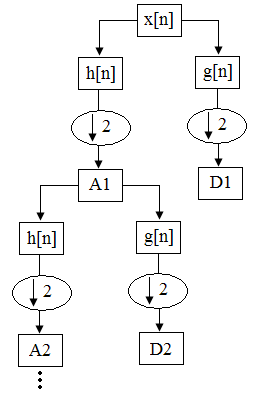
\includegraphics{image001.png}

Figure 1: Schematic representation of Multi-Resolution Analysis (MRA) 
\end{center}


\section{Program description}

$Protolize!$ has a main panel (Fig. 2) from where a set of interfaces (modules) is accessed, that makes possible an easy and intuitive use of the frequency analysis techniques. 
\begin{center}
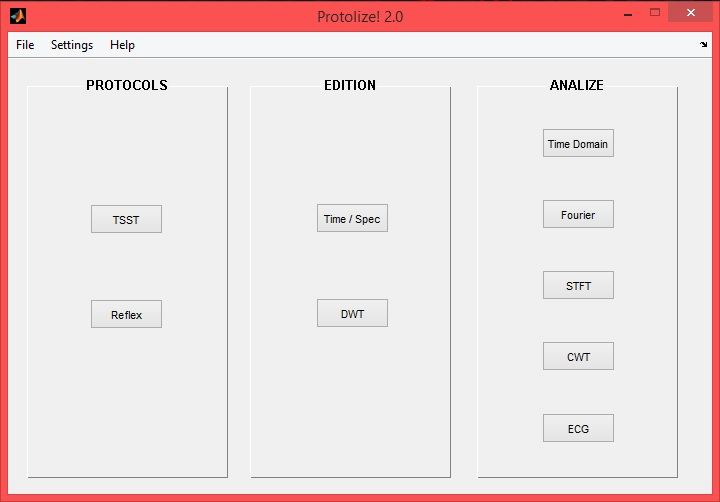
\includegraphics[width=15cm]{image002.jpg}

Figure 2: Main panel of $Protolize!$ with buttons to access each analysis module.
\end{center}
All modules were programmed to read ASCII files and to export to text or Excel files the data resulting from the analysis. Here we describe the main features offered by each module. 


The Fourier Module (Fig. 3) offers the following options:
\begin{itemize}
\item Process up to seven different signals simultaneously.
\item Calculate the power spectrum of each signal. 
\item Show, according to the user’s choice, besides the power spectrum, also the signals in the time domain for a better visual relationship between the two domains. 
\item As the module is focused in EEG signals, a power calculation of the main EEG rhythms delta ($0.5Hz-3.5Hz$), theta ($3.5Hz-7Hz$), alpha ($8Hz-13Hz$), beta ($13Hz-24Hz$) and gamma ($30Hz-70Hz$) was included.
\item The user can define a different band frequency for each EEG rhythm if necessary.
\item Select a specific time interval of the signal(s) analyzed in order to calculate the power spectrum only for that interval.
\end{itemize}
$$Insert Figure 3 about here$$


The STFT Module (Fig. 4) offers the following options:
\begin{itemize}
\item Choose between six different windows types: Hamming, Gaussian, Blackman, Hanning, Kaiser or Hann.
\item Define the time resolution by setting the window size and overlapping. 
\item Generate the spectrogram with a possibility of rotate it in three dimensions. 
\item Visualization of the power spectrum from each time interval separately.
\item Visualization of a specific frequency power trough time.
\end{itemize}
$$Insert Figure 4 about here$$


The CWT module (Fig. 5) offers the following options:
\begin{itemize}
\item Calculate the Continuous Wavelet Transform using one of ten different wavelets families (Haar, Daubechies, Symlets, Coiflets, Biorthogonal, R Biorthogonal, Meyer, Gaussian, Mexican, Morlet)
\item Choose the scale interval and resolution.
\item Pre-defined scale configuration in order to represent one of the EEG rhythms of interest. 
\item Plot separately the variation of one specific scale, selected by the user, through time.
\item Plot separately all scales values of one specific time selected by the user.
\item Scale/Pseudo-frequency converter.
\end{itemize}
$$Insert Figure 5 about here$$


The DWT Module (Fig. 6) offers the following options:
\begin{itemize}
\item Calculate the Discrete Wavelet Transform using one of six different wavelets families available. (Haar, Daubechies, Symlets, Coiflets, Biorthogonal, R Biorthogonal)
\item Decompose the signal defining one of the 10 first levels of resolution (Multi Resolution Analysis). 
\item View the coefficients or reconstruction of details and approximations at any calculated level. 
\item Edit the coefficients of any detail level or/and last approximation. 
\item Reconstruct the signal from details and last approximation after their edit process.
\end{itemize}
$$Insert Figure 6 about here$$


\section{System performance and examples}

To illustrate the system performance we used $Protolize!$ to detect the classical phenomenon of alpha block.  It is well know that during relaxing periods, with closed eyes, an increase in alpha rhythm power can be detected [15]. This increase is blocked in presence of visual or auditory stimuli. 

In order to reproduce and detect this phenomenon by using $Protolize!$, a set of EEG signals was collected, from 47 students of University of Brasilia, using an equipment Neuromap® (Neurotec®) model 40i and $Ag-AgCl$ electrodes located according to the 10-20 system in the positions $t3$ and $t4$. The impedances were kept under $5k\Omega$. The signal was acquired with a $256 Hz$ sample rate and band-pass filtered between $0.01 Hz$ and $100 Hz$ using Neuromap v.2.03 software. The study was approved by the Ethical Committee from the University of Brasilia, Faculty of Health Sciences. The signal contained three intervals of one minute each: the first and third intervals corresponded to time intervals where the subject was asked to relax and keep their eyes closed. At the second interval, the subject was asked to keep their eyes opened. Using the Fourier Module, the power of the alpha rhythm for each subject was calculated at each interval.  An ANOVA test to compare the alpha power at t3 electrode showed statistically significant differences between intervals ($F_{2,39}=5.88, p=0.006$). The Bonferroni test showed that the alpha power in the second (eyes opened) interval was significantly lower than first ($t=3.08, p=0.011$) and third ($t=2.83, p=0.022$) intervals (eyes closed). But there was no differences between the first and the third intervals ($t=0.198, p=1$). The same result was obtained for the t4 electrode. An ANOVA test showed differences between intervals ($F_{2,39}=8.143, p=0.001$) and Bonferroni showed differences between the first  ($t=3.523, p=0.003$) and third ($t=3.445, p=0.004$) intervals if compared with the second interval, but no differences between them ($t=0.141, p=1$) (Fig. 7).
\begin{center}
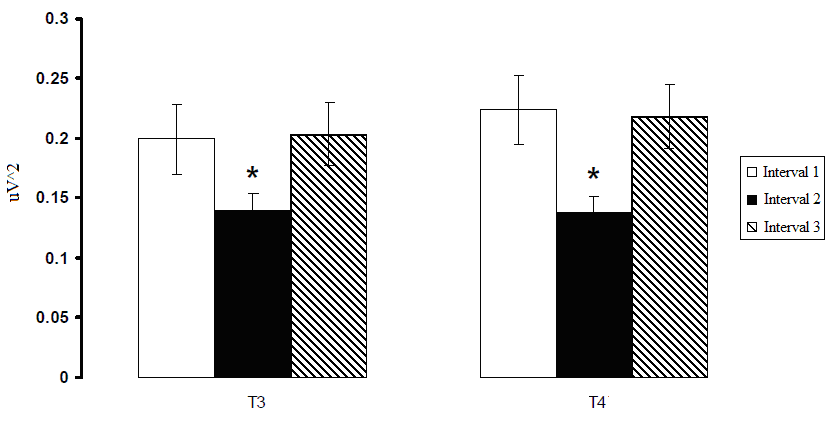
\includegraphics{image007.png}

Figure 7: Mean $pm$ SE of alpha power in each interval. * Differences statistically significantly between interval 2 (opened eyes) and intervals 1 and 3 (closed eyes)
\end{center}

\section{Hardware and software requirements}

To run $Protolize!$, Matlab® R2007b or newer is necessary and a computer with at least it $512MB$ RAM is recommended. The program was written using the Matlab basic functions, and the GUIDE, Signal Processing and Wavelets toolboxes.

\section{Advantages and availability}

$Protolize!$ is a powerful tool in frequency domain analysis. It allows noise reduction, main frequency components identification, calculation of main EEG rhythms power, time-frequency analysis and multi-resolution analysis. In spite of the pre-defined options for EEG analysis, Protolize! is not limited to this signal and can be used to analyze other kinds of signals as well. There are several computational tools for biological signal analysis commercially available [19] but normally they have a high cost or are linked to specific equipment or offer less analysis methods implemented. Protlize! is an open source, free distributed program available in GitHub through https://github.com/ishiikurisu/P2, making it a good option as a tool for biological signal processing. 

\section{Recomendations}

A pre-processing of the signal is desirable. Signals as EEG commonly have many artifacts produced by interference of signals such as electrocardiography and/or electrooculgraphy that can modify the results obtained. These artifacts also can be detected and minimized using techniques based in the methods offered by Protolize! [16,17] 

The use of STFT implies a compromise between time and frequency resolution. Choosing a very high time resolution by setting a window of very short duration leads to a decrease in the number of samples considered in the Fourier Transform calculation which could result in a low frequency resolution. 

It is recommended to consider effects as Gibbs phenomenon [18] to choose correctly the window to be used.

The calculation of CWT demands a high computational effort, thus it is not convenient to set a very high scales resolution (about $1/50$ of the scale interval desired). This could result in a high delay in the process and in an increase of memory needed to complete the calculation. 

\section{Acknowledgements}

This study was supported by grants from FINATEC and CNPq. S. Conde was the recipient of a CAPES fellowship. 

\section{References}

\begin{enumerate}

\item  S. W. Smith, (1998). The Scientist and Engineer's Guide to Digital Signal Processing. www.DSPguide.com. April 23, 2007.

\item  T. Miyashita, K. Ogawa, H. Itoh, Y. Arai, M. Ashidagawa, M. Uchiyama, Y. Koide,
T. Andoh, Y. Yamada, (2003). Spectral analyses of electroencephalography and
heart rate variability during sleep in normal subjects. Autonomic Neuroscience:
Basic and Clinical, 103(1-2), 114-120.

\item  M. Pedemonte, A. Rodriguez-Alvez, R.A. Velluti,  (2005). "Electroencephalographic
frequencies associated with heart changes in RR interval variability during
paradoxical sleep." Autonomic Neuroscience: Basic and Clinical, 123(1-2), 82-
86.

\item  N. V. Lutsyuk, E. V. Éismont, and V. B. Pavlenko, (2006). "Correlation of the Characteristics of EEG Potentials with the Indices of Attention in 12- to 13-Year-Old Children." Neurophysiology, 38(3), 209-216.

\item  L. V. Marcuse, M. Schneider, K. A. Mortati, K. M. Donnelly, V. Arnedo, and A. C. Grant, (2008). Quantitative analysis of the EEG posterior-dominant rhythm in healthy adolescents. Clinical Neurophysiology, 119(8), 1778-1781.

\item   K. M. Spencer, J. Polich, (1999). Poststimulus EEG spectral analysis and P300: Attention, task, and probability. Psychophysiology, 36(2), 220-232.

\item  P. J. Durka,  J. Zygierewics, H. Klekowicz, J. Ginter, K.J. Blinowska, (2004). On the statistical significance of event-related EEG desynchronization and synchronization in the time-frequency plane. Biomedical Engineering, IEEE Transactions, 51(7), 1167 - 1175.

\item  C. H. Yang,, Chi-Wan Lai, Hsien Yong Lai, T.B.J. Kuo, (2002). Relationship between electroencephalogram slow-wave magnitude and heart rate variability during sleep in humans. Neuroscience Letters, 329(2), 213-216.

\item  Q. R. Quiroga, O.A Rosso, and Basar, E. . (1999). Wavelets entropy: a measure of order in evoked potentials. Functional Neuroscience: Evoked Potentials and Magnetic Fields, 49, 299-303.

\item  Q. R. Quiroga, O.W. Sakowitz, E. Basar, and M. Schurmann, (2001 ). Wavelet Transform in the analysis of the frequency composition of evoked potentials. Brain Research Protocols, 8(1), 16-24.

\item  A. P. Bradley, and W. J. Wilson, (2004). On wavelet analysis of auditory evoked potentials. Clinical Neurophysiology, 115(5), 1114-1128.


\item  A. Subasi, (2005). Automatic recognition of alertness level from EEG by using neural network and wavelet coefficients. Expert Systems with Applications, 28(4), 701-711.

\item  D. Cvetkovic, E. D. Übeyli, and I. Cosic, (2008). Wavelet transform feature extraction from human PPG, ECG, and EEG signal responses to ELF PEMF exposures: A pilot study. Digital Signal Processing, 18(5), 861-874.

\item  S. G. Mallat, (1989). A Theory for Multiresolution Signal Decomposition: The Wavelet Representation. IEEE Transactions on Pattern Analysis and Machine Intelligence, 11(7), 674-693 

\item  F. W. Ganong, Alert Behavior, Sleep \& the Electrical Activity of the Brain. In: Medical Physiology, 2005. MacGraw-Hill, 22th Edition, Chapter 11, 192-201

\item  D. V. Moretti, F. Babiloni, F. Carducci, F. Cincotti, E. Remondini, P. M. Rossini, S. Salinari, and C. Babiloni, (2003). Computerized processing of EEG-EOG-EMG artifacts for multi-centric studies in EEG oscillations and event-related potentials. International journal of psychophysiology 47(3), 199–216.

\item  A. Gutiérrez, M. Lara, and P. R. Hernández, (2005). Evaluación de un Detector de Complejo QRS Basado en la Wavelet de Haar, usando las Bases de Datos MIT-BIH de Arritmias y Europea del Segmento ST y de la Onda T. Computación y Sistemas, 8(4), 293-302

\item  T. Masters, Neural, Novel \& Hybrid Algorithms for Time Series Prediction, John 
Wiley \& Sons, Inc., USA,1995.

\item  M. A. Guevara, J. Ramos, M. Hernandez-Gonzalez, and M. Corsi-Cabrera, (2005). FILDIG: A program to filter brain electrical signals in the frequency domain. Computer Methods and Programs in Biomedicine, 80, 165-172


\end{enumerate}

\end{document}